\section{Auswertung / Fazit}


\begin{frame}{Analyse der Ergebnisse - Güte}
    \begin{itemize}
        \item Überaschend: Fast-Anchor-Clustering schlechter?
        \item Abstand der Lösungen korreliert mit Dimensionalität der Daten
        \item Zusätzlich noch langsamer
    \end{itemize}
\end{frame}


\begin{frame}{Analyse der Ergebnisse - Güte}
    \begin{center}
        \begin{minipage}[t]{0.55\textwidth}
            \begin{center}
                \begin{large}
                    Fast-Anchor-Clsutering mit Max-Linie
                \end{large} 
            \end{center}   
            %\vspace{-\baselineskip} % Move image to the top
            
\includegraphics[width=\textwidth]{fig/Fast-Anchor Edge-Case/Edge-Case Curve.jpg}
        \end{minipage}
    \end{center}
\end{frame}











\begin{frame}{Probleme von Fast-Anchor-Clustering}
    \begin{minipage}[t]{0.55\textwidth}
        \begin{itemize}
            \item Für Fairlet-Radius nur Ankerabstand relevant
            \item $\rightarrow$ Unterschwellig größere Fairlets möglich
            \item \quad $\rightarrow$ Beide Fairlets haben Kennradius $a$
        \end{itemize}
    \end{minipage}
    \hfill
    \begin{minipage}[t]{0.44\textwidth}
        \vspace{-\baselineskip} % Move image to the top
        % Beispiel Flusserstellung
        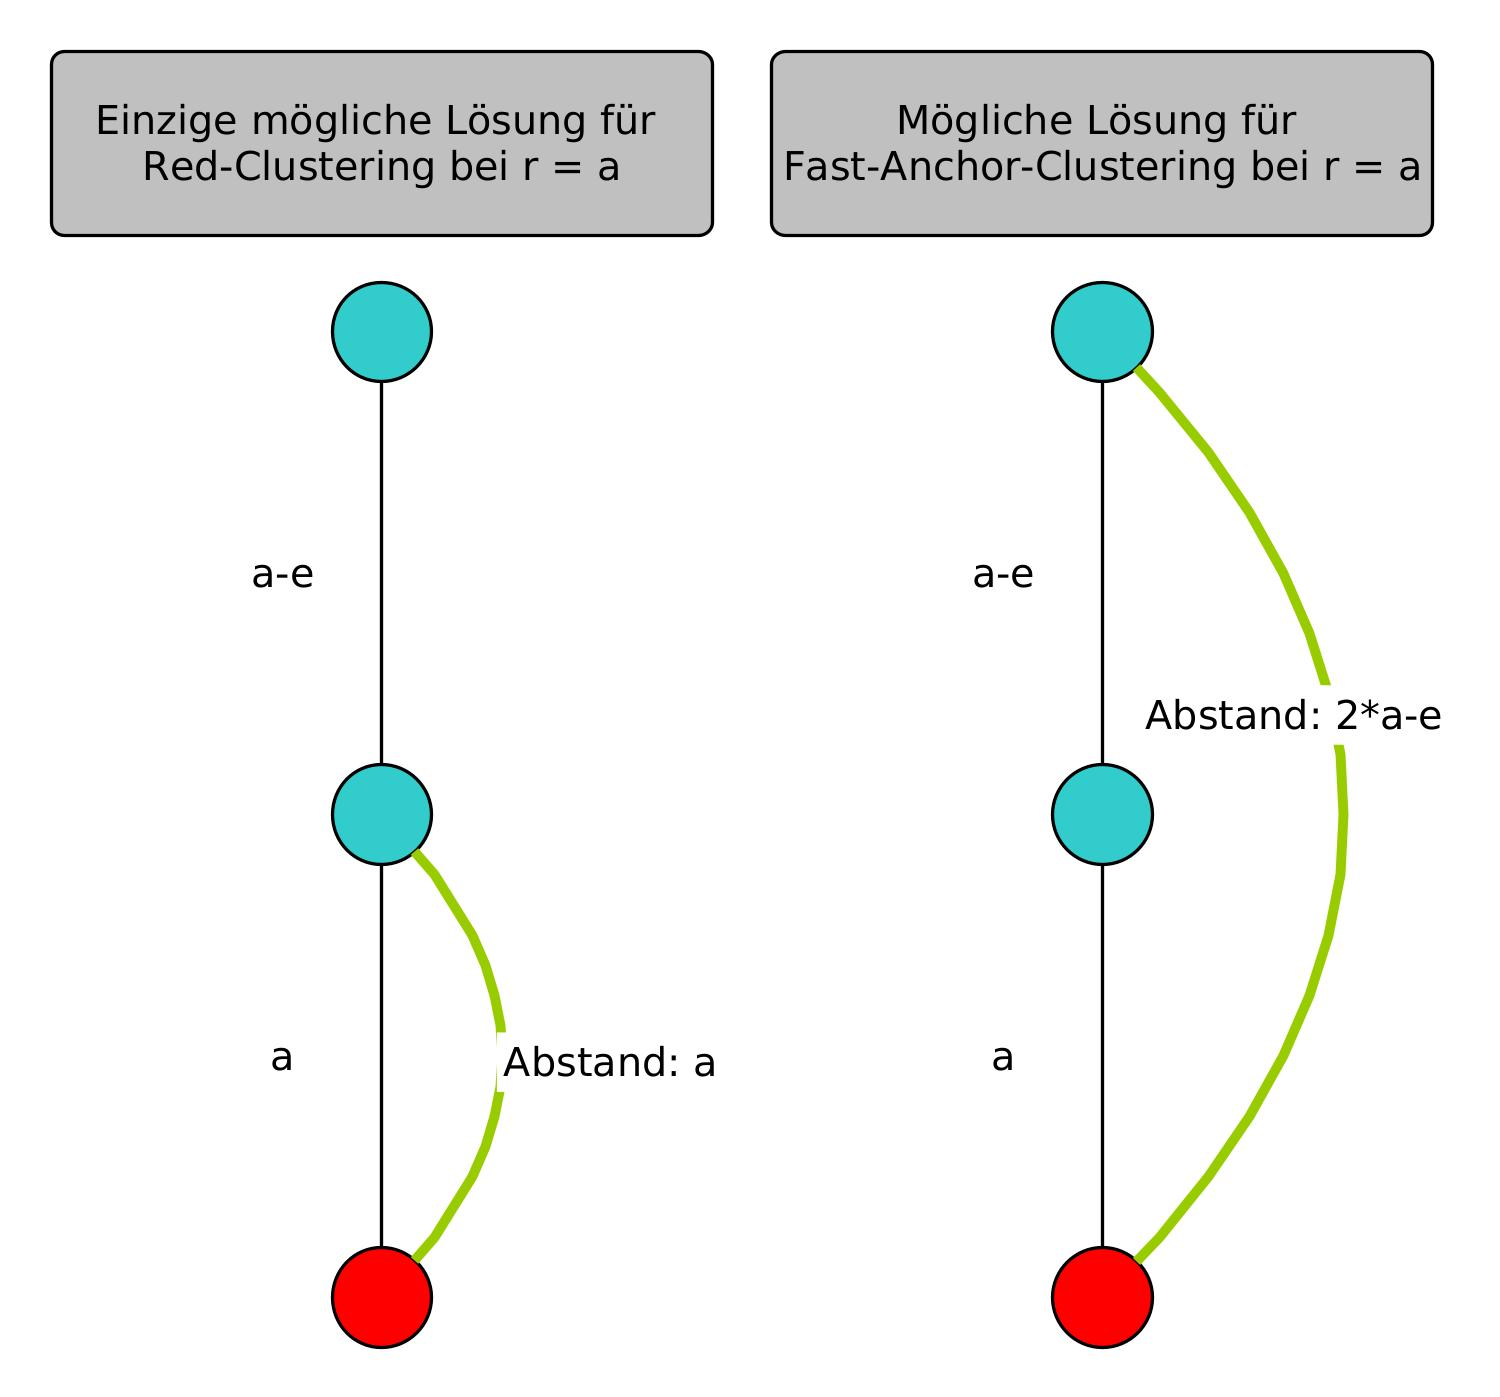
\includegraphics[width=\textwidth]{fig/Fast-Anchor Edge-Case/Fast-Anchor worse Fairlet.jpg}
    \end{minipage}
\end{frame}











\begin{frame}{Probleme von Center-Awareness}
    \begin{center}
        \begin{minipage}[t]{0.4\textwidth}
            \begin{large}
                \begin{center}
                    Fall k = 3
                \end{center}
            \end{large}        
            %\vspace{-\baselineskip} % Move image to the top
            
\includegraphics[width=\textwidth]{fig/Fast-Anchor Edge-Case/Bigger Cluster Edge-Case k=3.jpg}
        \end{minipage}
    \end{center}
\end{frame}

\begin{frame}{Probleme von Center-Awareness}
    \begin{center}
        \begin{minipage}[t]{0.4\textwidth}
            \begin{large}
                \begin{center}
                    Fall k = 4
                \end{center}
            \end{large}        
            % \vspace{-\baselineskip} % Move image to the top
            
\includegraphics[width=\textwidth]{fig/Fast-Anchor Edge-Case/Bigger Cluster Edge-Case k=4.jpg}
        \end{minipage}
    \end{center}
\end{frame}














\begin{frame}{Mögliche Verbesserung}
    \begin{itemize}
        \item Laufzeit
        \begin{itemize}
            \item redundante Berechnungen redunzieren
            \item parallele Berechnungen
        \end{itemize}
        \item Kosten
        \begin{itemize}
            \item Gonzalez Optimieren
            \item nicht Center-Aware Arbeiten
        \end{itemize}
        \item Analyse
        \begin{itemize}
            \item mehr/diversere Daten
            \item optimale Lösungen zum Vergleich
        \end{itemize}
    \end{itemize}
\end{frame}




